\hypertarget{st}{\subsubsection{Storage contracts}}
In this section we will illustrate the storage contracts. As mentioned before the storage contracts are immutable because they store all the critical data. When a contract is upgraded a new version of itself (using inheritance) is deployed, and all its state variables are new. To avoid data loss, all the data stored in the previous version of the contract should be copied into the new version. This copy is very expensive, due to high costs of writing on storage variables.\\
To avoid that, storage contracts implement don't implement any kind of business logic. Their purpose is to store data and to allow specific contracts to modify their state. For data retrieval, on the other hand, the are no limitations because getter methods don't modify the state of storage contracts.
All storage contracts inherit from \texttt{Authorizable} in order to use the \texttt{onlyAuthorized} modifier in the setter methods.
\paragraph*{Note: struct in the storage contracts}
All contracts, except for \texttt{VatStorage}, in their struct have three state variables: \texttt{hashIpfs, hashFunction} and \texttt{hashSize}, which represent the \texttt{IPFS CID} used to locate additional data on the \texttt{IPFS} network such as name and surname for users. The choice to separate critical data from additional data has been made in order to optimize storage costs.
\pagebreak
\paragraph{UserStorage}\mbox{}\\

\noindent This contract maintain the VAT amount of every business for every quarter. Each time a business buy or sell some products, the vat amount of each product is added or subtracted to the amount in this contract. If the product is sold, its VAT is added, whereas if the product is sold the vat is subtracted. \\

\noindent This contract stores all the critical data of the users. 
\begin{figure}[H]
	\centering
	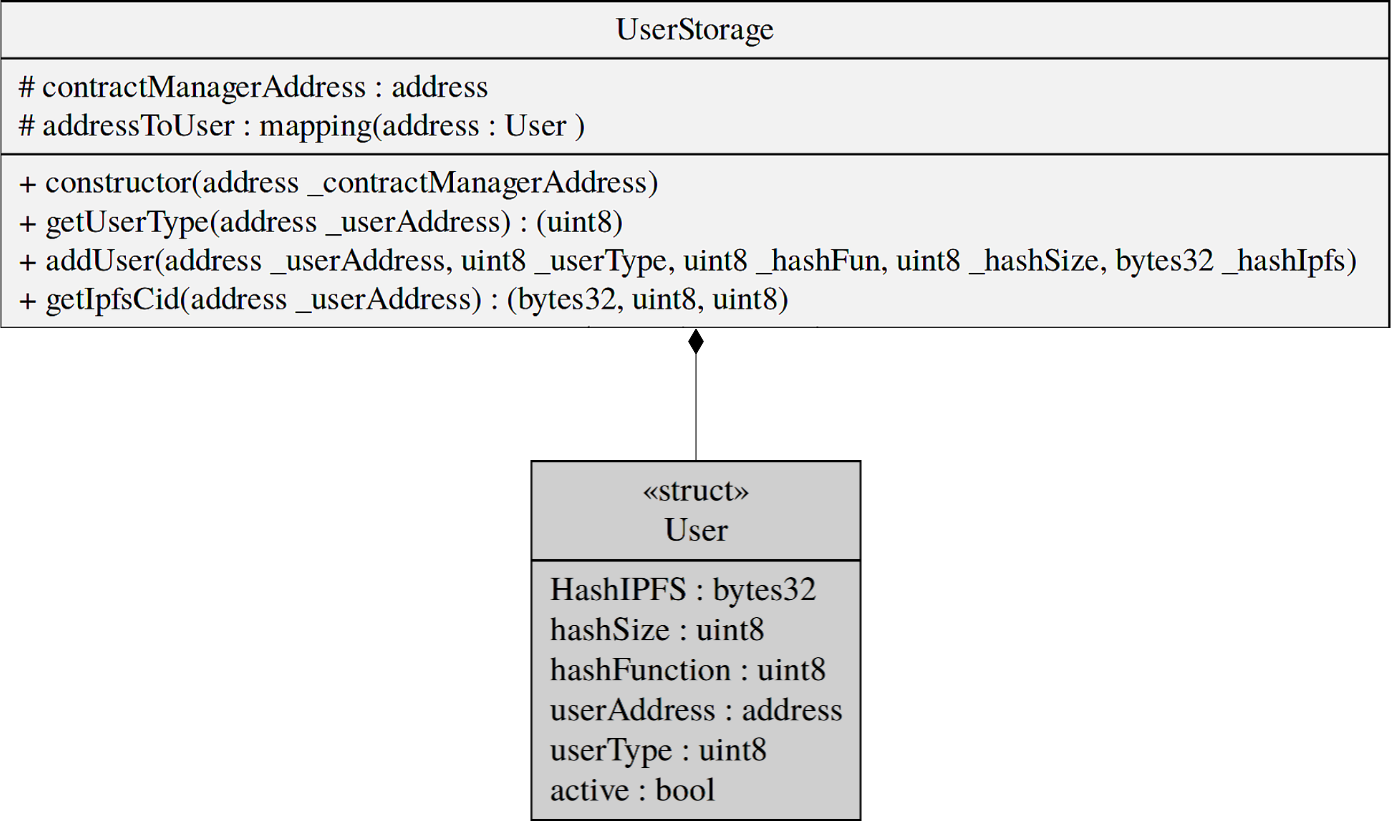
\includegraphics[scale=0.25]{res/images/solidity/userstorage.png}
	\caption{class diagram of the UserStorage contract}
\end{figure}
\pagebreak
\paragraph{ProductStorage}\mbox{}\\

\noindent The \texttt{ProductStorage} contract stores all the data needed to be secured (e.g. net price). Furthermore, the contract defines all methods used to maintain the data. 
\begin{figure}[H]
	\centering
	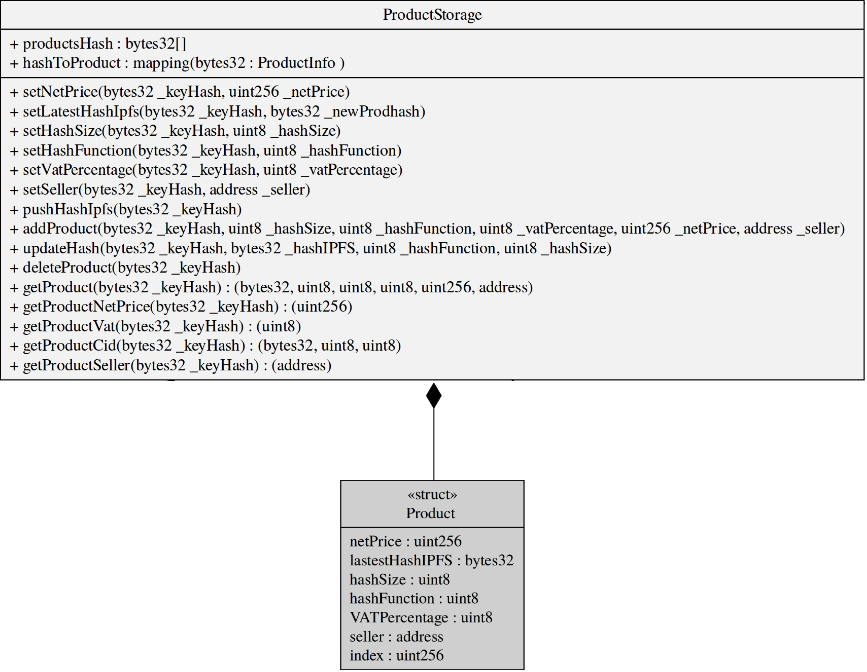
\includegraphics[scale=0.45]{res/images/solidity/productstorage.png}
	\caption{class diagram of the ProductStorage contract}
\end{figure}
\pagebreak
\paragraph{VatStorage}\mbox{}\\

\noindent This contract maintains the VAT amount of every business for every quarter. Each time a business buys or sell some products, the VAT amount of each product is added or subtracted to the amount in this contract. If the product is sold, its VAT is added, while if the product is sold the VAT is subtracted. \\
\texttt{VatStorage} has an array of map keys in order to iterate the map and enumerate its elements. 

\begin{figure}[H]
	\centering
	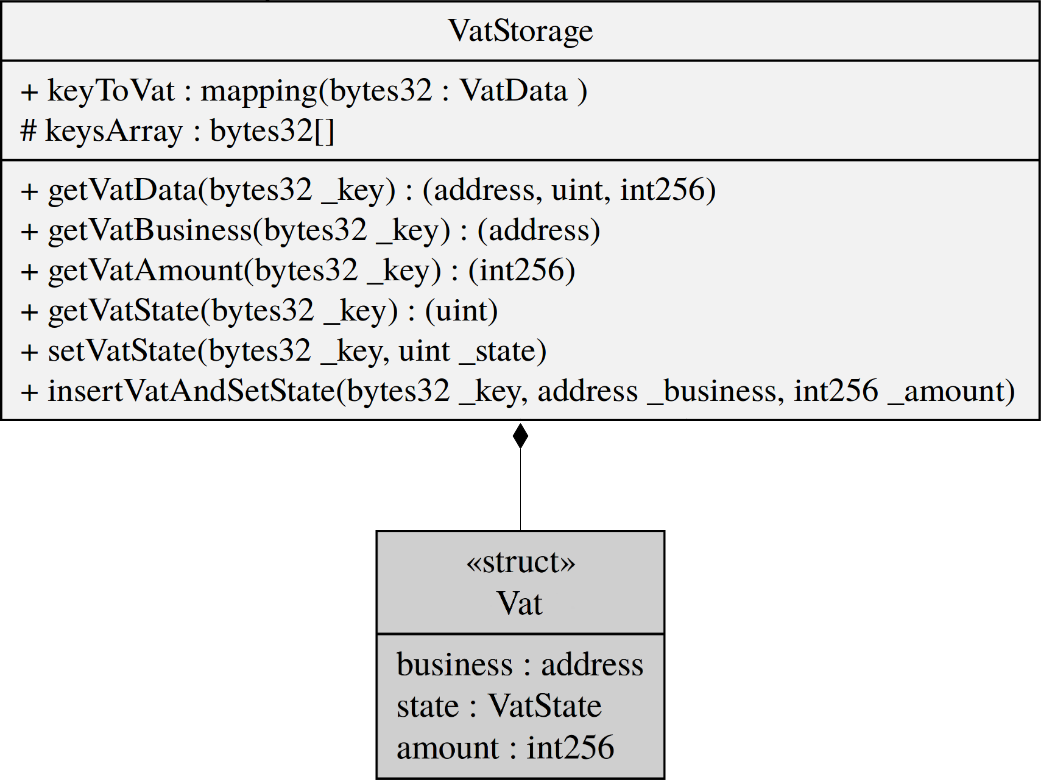
\includegraphics[scale=0.30]{res/images/solidity/vatstorage.png}
	\caption{class diagram of the VatStorage contract}
\end{figure}
\pagebreak

\paragraph{OrderStorage}\mbox{}\\

\noindent This contract stores all the information of an order. In its struct are saved also the product keys (\texttt{productsHash}) of the order.
\begin{figure}[H]
	\centering
	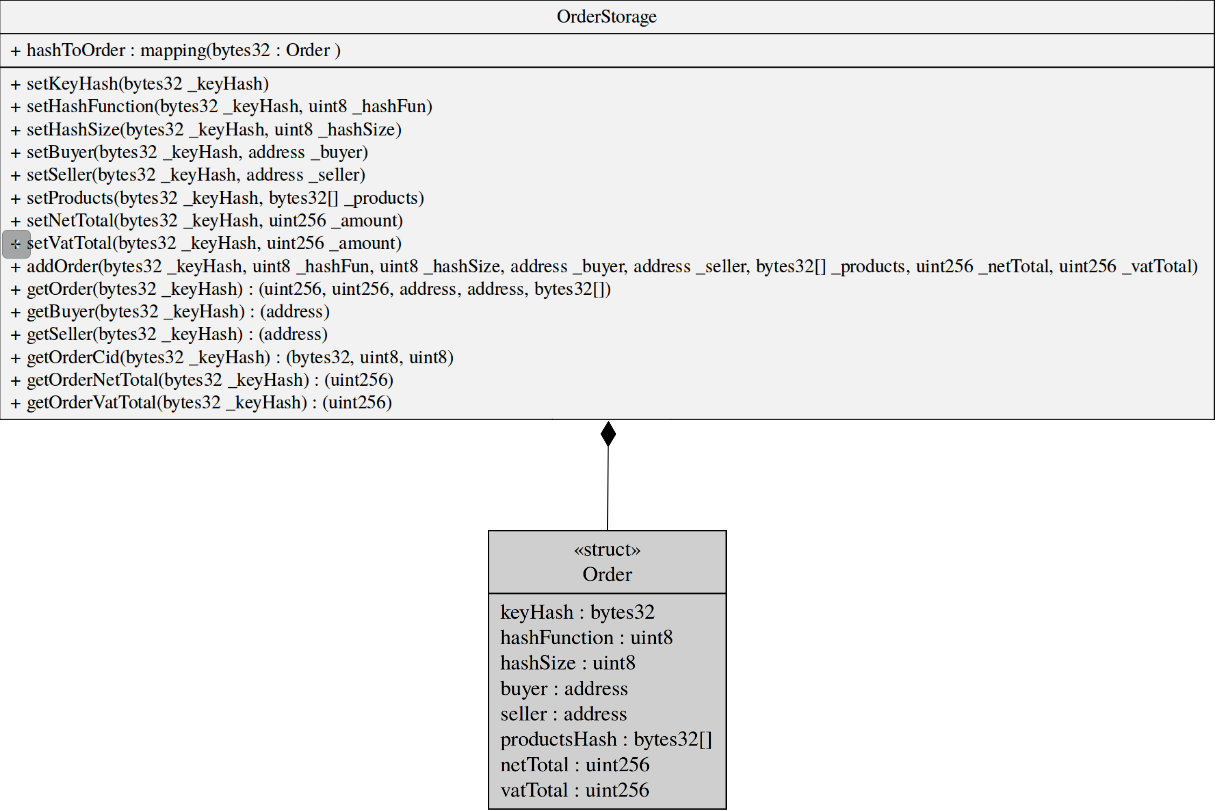
\includegraphics[scale=0.35]{res/images/solidity/orderstorage.png}
	\caption{class diagram of the OrderStorage contract}
\end{figure}